%第3章

\section{感染症予防サポートシステムの概要}

本節では,感染症予防サポートシステムの目的,要求仕様及び概要を述べる.

まず,今回作成する感染症予防サポートシステムの目的としては,感染症予防の観点から感染リスクのレベルを通知するとともに,感染リスクを軽減する環境づくりをサポートすることである.この目的を基にし,システムは,下記の2点の要求事項を満たす必要がある.

\begin{itemize}
\item 室内環境が測定できること.
\item 設定した感染リスクの基準に従って通知ができること.
\end{itemize}

上述の「室内環境が測定できること」という要求事項は,二酸化炭素濃度,温湿度,室内滞在人数が測定できるということである.
また,上述の「設定した感染リスクの基準に従って通知ができること」という要求事項は,ユーザーに対して,ブザーやLEDを用いて能動的に環境値が基準値を超えていることを知らせることである.

以上の要求事項を満たすためには,本研究では,Webカメラと各種センサを室内に設置することで,室内の二酸化炭素の濃度値,温湿度値,在室人数などの室内環境をリアルタイムにモニタリングを行い,室内の感染リスクを自動的に解析し,室内外のユーザーに感染リスクを通知する感染症予防サポートシステムを提案する.

本研究において対象とする部屋は,学校の教室など,数人から数十人程度が利用する部屋とする.


本研究で提案するシステムを使用する流れを図\ref{summary1}に示す.


\begin{figure}[htbp]
\centering
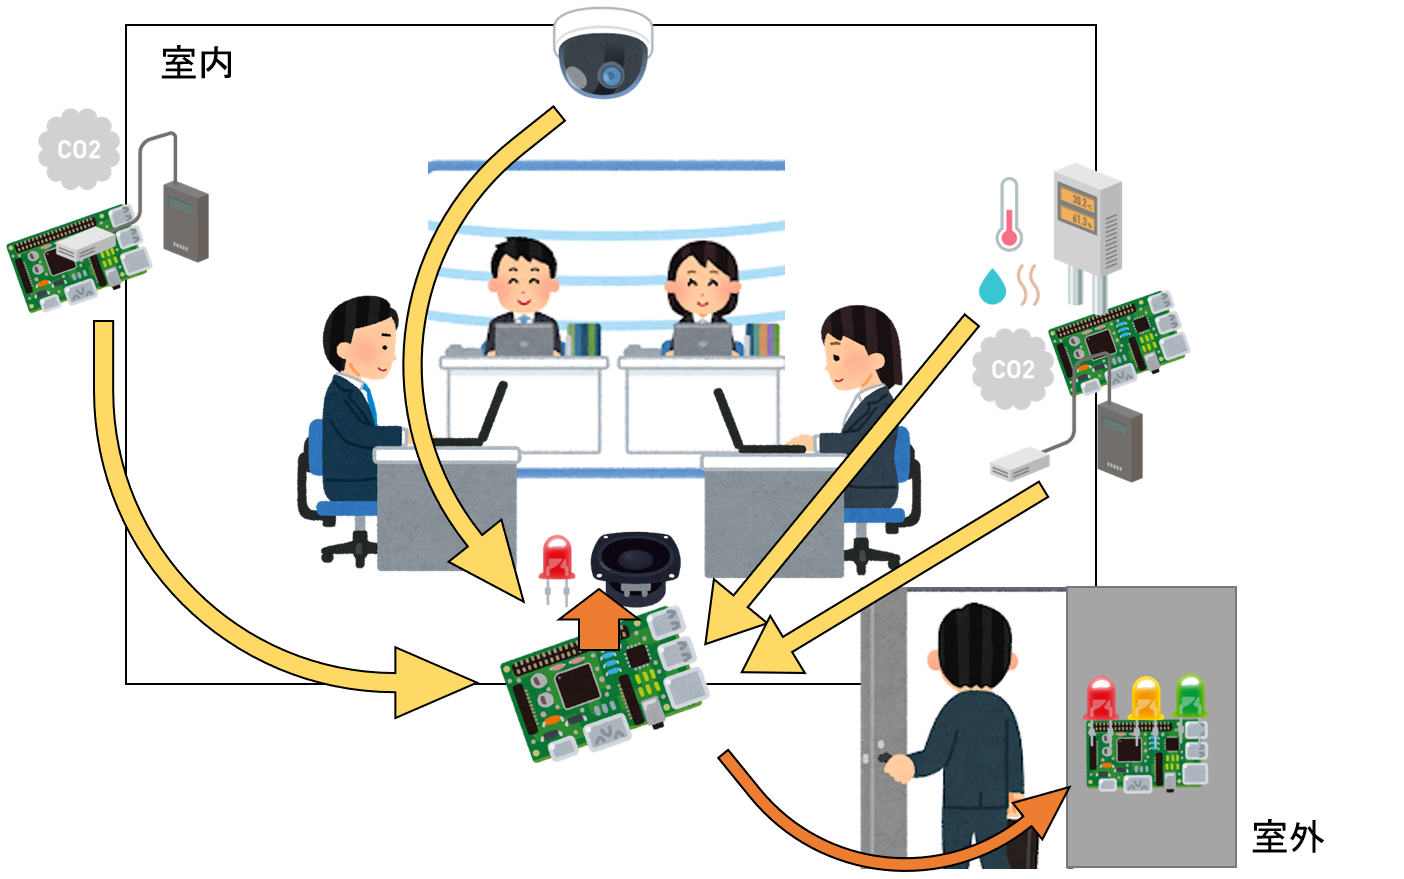
\includegraphics[width = 15cm]{./system.eps}
\caption{システム全体の流れ}
\label{summary1}
\end{figure}


まずパソコン上で部屋の大きさを入力することで,部屋に滞在できる上限人数が設定され,標準警戒レベルでの室内モニタリングが開始される.各種センサやWebカメラでモニタリングした結果を評価し,LEDやブザーを用いて室内外のユーザーに通知する.使用するハードウェア,ソフトウェアの役割を以下の図\ref{summary2}に示す.


\begin{figure}[htbp]
\centering
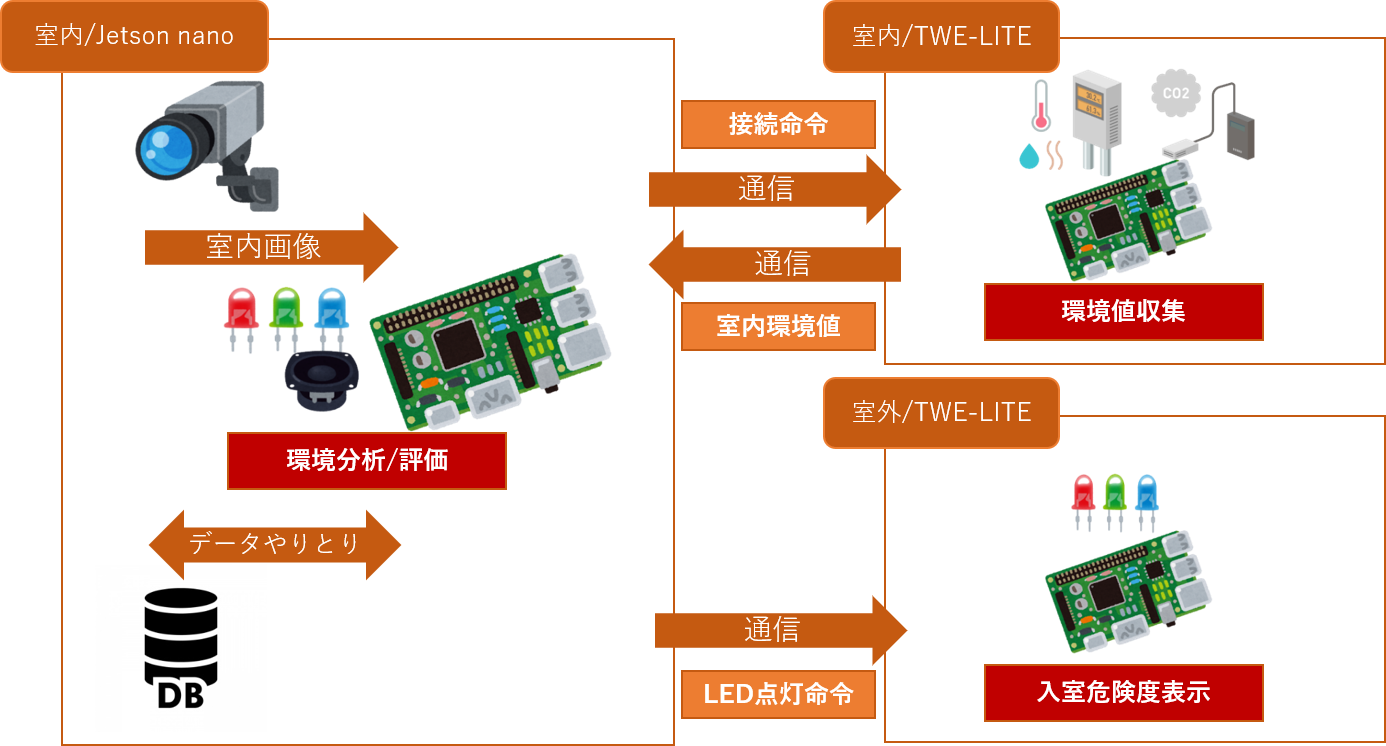
\includegraphics[width = 15cm]{./system2.eps}
\caption{システムのイメージ図}
\label{summary2}
\end{figure}


感染症予防サポートシステムはデータの分析・評価を行うJetson nano,データ収集を行うセンサデバイス,および入室危険度を表示する室外デバイスから構成される.各種センサデバイスから室内の温湿度や二酸化炭素濃度の情報を,Webカメラから室内の画像を取得し,その情報をJetsonへ送信する.Jetsonではカメラ画像から室内の人数を判別し,その他の室内環境情報と合わせて警戒レベル・入室危険度を決定して,室内に向けてアラートを発すると同時に室外デバイスに入室危険度を送信する.室外デバイスは受信した入室危険度に応じてLEDを点灯する.


なお,本システムの開発は,センサデバイスの作成を稲田一輝が,人数判別部を伊藤大輝が,データ管理・分析・評価や室内アラートの制御を掛水誠矢が,室外表示デバイスの作成を小田恵吏奈が担当した.